\begingroup
	\pgfdeclarelayer{background layer}
	\pgfsetlayers{background layer,main}
	\tikzstyle{zero}=[circle,draw=black,fill=white,inner sep=0pt,minimum size=2.5mm]
	\tikzstyle{one}=[circle,draw=black,fill=black,inner sep=0pt,minimum size=2.5mm]
	\tikzstyle{two}=[circle,draw=black,fill=gray,inner sep=0pt,minimum size=2.5mm]
		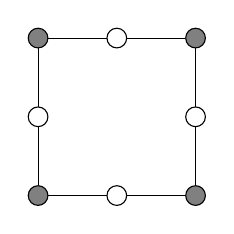
\begin{tikzpicture}
			\node (1) at (-1,-1) [two] {};
			\node (a) at (1,-1) [two] {};
			\node (0) at (1,1) [two] {};
			\node [white] (b) at (-1,1) [two] {};
			\node at (1,0) [zero] {};
			\node at (-1,0) [zero] {};
			\node at (0,1) [zero] {};
			\node at (0,-1) [zero] {};
			\begin{pgfonlayer}{background layer}
				\draw (1) -- (a);
			\draw (1) -- (b);
			\draw (a) -- (0);
			\draw (b) -- (0);
			\end{pgfonlayer}
		\end{tikzpicture}
	%\label{fig:eg_universal_no_simplicial_map}	
\endgroup